\Problem{Demo Problem}

\Statement

\paragraph{Abstract.}

This a demo problem whose statement includes many elements that can be used in Jutge.org. 
Please refer to its source code to see how to include these elements in your own problem statements.

\medskip

Problems statements are written in \LaTeX, which allows for great flexibility and high-quality typesetting.
Resulting statements are rendered in PDF, HTML, Markdown, and plain Text formats. Jutge.org aims to have
a consistent appearance across all formats, although some features may vary depending on the capabilities of each format.


\paragraph{Text.}

Regular text is just written as \LaTeX. 
It is important to remember to separate paragraphs with the \verb|\medskip| macro.

\medskip

Lorem ipsum dolor sit amet, consectetur adipiscing elit. Vivamus lacinia odio vitae vestibulum vestibulum. 
Cras venenatis euismod malesuada. 
Nullam ac erat ante. 
Sed vel lacus id mauris dapibus facilisis. 
Nam euismod, tortor nec pharetra ultricies, ante erat imperdiet velit, nec laoreet enim lacus a velit.

\medskip

Latin accents and special characters are supported out of the box: Bé, sí, allà algú dirà: «Què farà l'avió demà?» "Potser" vindrà ràpid, però demanarà atenció. 
Greek letters works well: Καλημέρα, πώς είστε σήμερα.
Asiatic languages work well in HTML but not in PDF: 你好,很高兴认识你。「はじめまして、よろしくお願いします。」.
Emojis work well in HTML but not so-so in PDF: ⚠ 😀 .

\paragraph{Maths.}

The use of mathematical expressions is also supported. 
They can be included inline, like the famous $E = mc^2$ formula or simply as $\sqrt x$, or as separate displayed equations. 
For example, we can write the quadratic formula as follows:

\[
    x = \frac{{-b \pm \sqrt{{b^2 - 4ac}}}}{{2a}}
\]

or express the Pythagorean theorem:

\[
    a^2 + b^2 = c^2
\] 

The rendering of these expressions will use MathML in the HTML version, ensuring very nice results. 
In the Text and Markdown versions, mathematical expressions will be represented using some unicode symbols or in LaTeX format. 


\paragraph{Conditional rendering.}

Some parts of the statement can be conditionally included depending on the output format.

\medskip

\begin{latexonly}
    This text is only included in the PDF version of the statement.
\end{latexonly}

\begin{htmlonly}
    This text is only included in the HTML, Markdown and Text versions of the statement.
\end{htmlonly}



\paragraph{Images.}

Images can also be included in the statement. For instance, here are two images of the famous bell tower of La Torrassa:

\begin{center}
\includegraphics[width=3cm]{campanar}
\qquad
\includegraphics[width=5cm]{campanar}
\end{center}

Available formats are PNG, JPG, PDF, BMP and EPS. SVG is also supported in HTML but not in PDF. Prefer vector formats (PDF, EPS, SVG) whenever possible to ensure the best quality at any size, and use PNG or JPG only for raster and photographic images.

\medskip

Use conditional rendering to include different images depending on the output format:

\begin{center}
\begin{latexonly}
    
\includegraphics[width=3cm]{jutge.png}
\end{latexonly}
\begin{htmlonly}
    
\includegraphics[width=3cm]{jutge.svg}
\end{htmlonly}
\end{center}

In the HTML version, figures will be embedded in the document, ensuring compatibility across different browsers without relying on external files. In the Text and Markdown versions of the statement, images will be represented by their filenames enclosed in square brackets. Unfortunately, Pandoc does not honor alignment of images.


\paragraph{Code.}

Code snippets can be included using the \textbf{listings} package. Here is a simple Python code example:

\begin{lstlisting}[language=Python, xleftmargin=0.75cm]
import yogi 

a = yogi.read(int)
b = yogi.read(int)
print(a + b)
\end{lstlisting}

and here is a C++ code example:

\begin{lstlisting}[language=C++, xleftmargin=0.75cm]
#include <iostream>
using namespace std;

int main() {
    int a, b;
    cin >> a >> b;
    cout << a + b << endl;
    return 0;
}
\end{lstlisting}

The listings package supports many programming languages and produces nicely formatted code both in PDF and HTML statements.

\medskip

\lstset{language=C++}
Code snippets can also be included inline: \lstinline|if (found) cout << pos;|.
In this case, it was necessary to use \verb|\lstset{language=C++}| to set the language.


\paragraph{Inline code deprecations.}

The former use of at signs (@) and vertical bars (|) to include inline code snippets is deprecated because \textbf{pandoc} does not support it and introduced conflicts with other packages. You will have to replace them with \verb|\lstinline| or with \verb|\verb|| as shown above. Statements with at signs for inline listings can be automatically converted using \texttt{jtk convert transform-at-signs}.


\paragraph{Hyperlinks.}

Hyperlinks can be included in the statement using the \textbf{hyperref} package. 
For example, visit \href{https://jutge.org}{Jutge.org} for more information.
In the PDF and HTML versions, the link will be clickable, in the Markdown version, the URL will be displayed as required, but the Text version will only show the link text (Why? Can we fix it?).

\medskip
In addition, the \verb|Link| macro is provided to include links to other Jutge.org problems: 
See the Hello World problem \Link{P68688}. Adding the language suffix is not recommended.


\paragraph{Colors.}

Colors can be used in the statement using the \textbf{color} package. 
For instance, \textcolor{red}{this text is red}, \textcolor{blue}{this text is blue}, and \textcolor{green}{this text is green}.
Of course, colors are not supported in the Text and Markdown versions of the statement.


\paragraph{Columns.}

The statement can also include multiple columns using the \textbf{multicol} package.
Here is an example with two columns:

\begin{multicols}{2}

Lorem ipsum dolor sit amet, consectetur adipiscing elit, sed do eiusmod tempor incididunt ut labore et dolore magna aliqua. Ut enim ad minim veniam, quis nostrud exercitation ullamco laboris nisi ut aliquip ex ea commodo consequat. Duis aute irure dolor in reprehenderit in voluptate velit esse cillum dolore eu fugiat nulla pariatur. Excepteur sint occaecat cupidatat non proident, sunt in culpa qui officia deserunt mollit anim id est laborum

\end{multicols} 

This is shown in the PDF version only, as multiple columns are not supported in HTML, Text, or Markdown.


\paragraph{PS Tricks.}

PS Tricks figures can also be included in the statement but this is discouraged as it is not supported in HTML. Here is a simple example:

\begin{center}
\begin{pspicture}(0,0)(2,2)
\psline{->}(0,0)(2,2)
\pscircle(1,1){1}
\end{pspicture}
\end{center}

\paragraph{Tikz.}

Tikz figures can also be included in the statement but this is discouraged as it is not supported in HTML. Here is a simple example:

\begin{center}
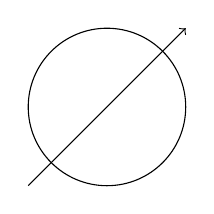
\begin{tikzpicture}
\draw[->] (0,0) -- (2,2);
\draw (1,1) circle (1cm);
\end{tikzpicture}
\end{center}

\paragraph{Chessboards.}

Chessboards can also be drawn in the statement using the \texttt{chessboard} package but this is discouraged as they are not supported in HTML.

\begin{center}
    \chessboard[setpieces={Ke1, Qd1, Ra1, Rh1, Bc1, Bf1, Nb1, Ng1,
    ke8, qd8, ra8, rh8, bc8, bf8, nb8, ng8},
    showmover=false]
\end{center}    



\Input

The Input section describes the format of the input data that your program will receive.

\Output

The Output section describes the format of the output data that your program must produce.

\Observation

There are a bunch of sectioning macros that can be used to include additional information in the statement:

\begin{itemize*}
    \item \verb|\Observation|
    \item \verb|\Observations|
    \item \verb|\Example|
    \item \verb|\Precondition|
    \item \verb|\Scoring|
    \item \verb|\Scores|
    \item \verb|\Hint|
    \item \verb|\Interface|
    \item \verb|\ObservationElastic|
    \item \verb|\ObservationElasticII|
    \item \verb|\ObservationNoMain|
    \item \verb|\Solution|
\end{itemize*}

These are localized automatically depending on the language of the problem.

\medskip

The following macros configure the listings package used to display code snippets according to the some programming languages:

\begin{itemize*}
    \item \verb|\UseCPP|
    \item \verb|\UsePython|
    \item \verb|\UseHaskell|
    \item \verb|\UseClojure|
\end{itemize*}


\medskip

Interface macros are provided to describe possible interfaces that depend on the programming language used (we plan to improve this in the future):

\Interface
\begin{tabular}{rl}
C++ &
\begin{lstlisting}[language=C++]
    int factorial(int n);
\end{lstlisting}
\\
C &
\begin{lstlisting}[language=C]
    int factorial(int n);
\end{lstlisting}
\\
Java &
\begin{lstlisting}[language=Java]
    public static int factorial(int n);
\end{lstlisting}
\\
Python &
\begin{lstlisting}[language=Python]
    factorial(n)  # returns int
\end{lstlisting}
\\
&
\begin{lstlisting}[language=Python]
    factorial(n: int) -> int
\end{lstlisting}
\end{tabular}

\bigskip

Scoring macros are provided to describe how the problem will be scored (you also need to provide a matching \texttt{scores.yml} file!):

\Scoring

\Score{Case A}{20}{Easy inputs.}
\Score{Case B}{30}{Medium inputs.}
\Score{Case C}{50}{Hard inputs.}


\medskip

Macros for including sample inputs and outputs are also provided:

\begin{itemize*}
    \item \verb|\Sample|
    \item \verb|\SampleOneCol|
    \item \verb|\SampleTwoCol|
    \item \verb|\SampleSession| (uses \verb|sample.dt| file)
\end{itemize*}

